\documentclass{article}
\usepackage{tikz}
\usepackage{amsmath,amsthm,amssymb}
\begin{document}
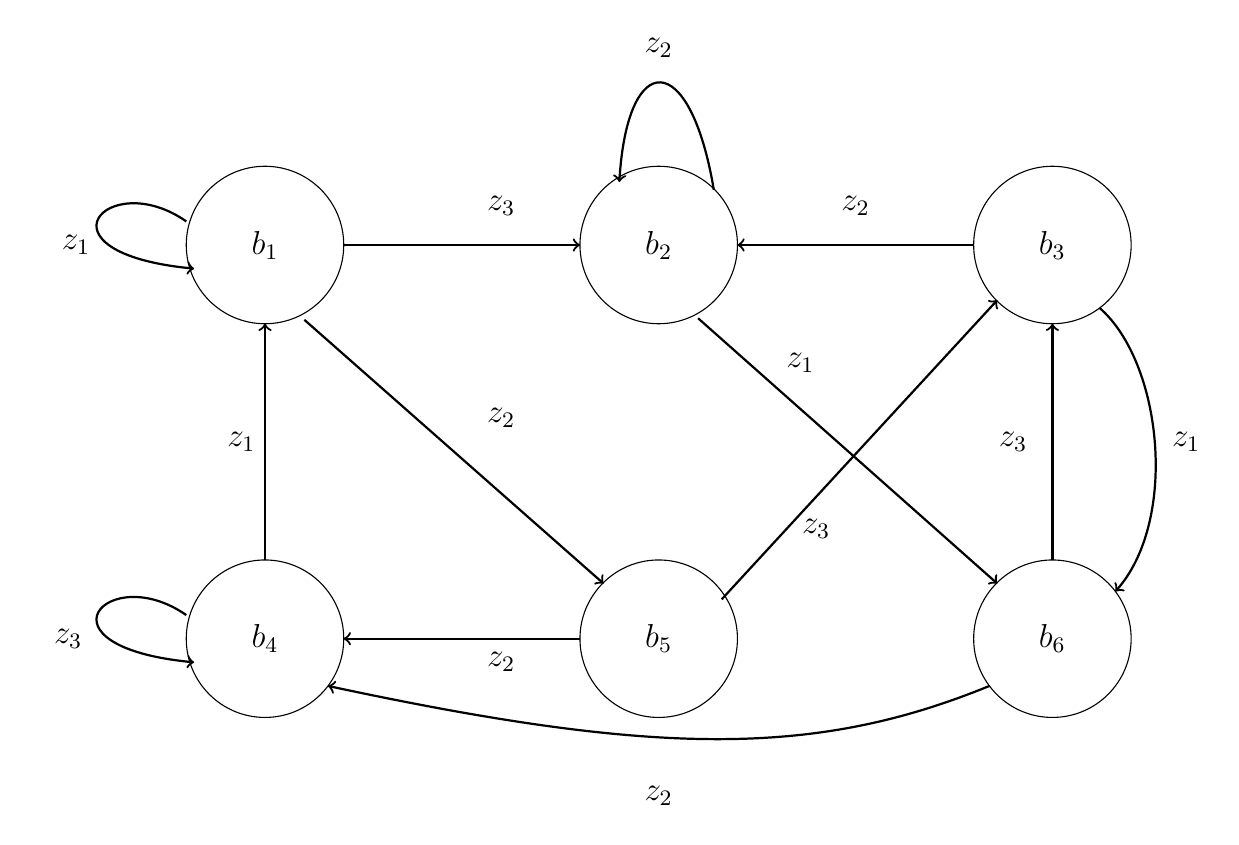
\begin{tikzpicture}

\large
\draw[thick, ->] (4.8,-4.5) -- (8.3,-0.7);
\draw[thick, ->] (-0.5,-0.95) -- (3.3,-4.3);
\draw[thick, ->] (4.5,-0.93) -- (8.3,-4.3);
\draw[thick, ->] (0,0) -- (3,0);
\draw[thick, ->] (-1,-4) -- (-1,-1);
\draw[thick, ->] (3,-5) -- (0,-5);
\draw[thick, <-] (5,0) -- (8,0);
\draw[thick, ->] (9,-4) -- (9,-1);
\draw [thick, ->] (-2,0.3) .. controls (-3,1) and (-4,-0.1) .. (-1.9,-0.3);
\draw [thick, ->] (-2,-4.7) .. controls (-3,-4) and (-4,-5.1) .. (-1.9,-5.3);
\draw [thick, ->] (4.7,0.7) .. controls (4.4,2.5) and (3.6,2.5) .. (3.5,0.8);
\draw [thick, ->] (9.6,-0.8) .. controls (10.4,-1.5) and (10.6,-3.5) .. (9.8,-4.4);
\draw [thick, ->] (8.2,-5.6) .. controls (6,-6.5) and (4,-6.5) .. (-0.2,-5.6);
\draw(-1,0) circle (1);
\draw (-1,0) node {$b_1$};
\draw(-1,-5) circle (1);
\draw (-1,-5) node {$b_4$};
\draw(4,-5) circle (1);
\draw (4,-5) node {$b_5$};
\draw(4,0) circle (1);
\draw (4,0) node {$b_2$};
\draw(9,0) circle (1);
\draw (9,0) node {$b_3$};
\draw(9,-5) circle (1);
\draw (9,-5) node {$b_6$};
\draw (-3.4,0) node {$z_1$};
\draw (-1.3,-2.5) node {$z_1$};
\draw (10.7, -2.5) node {$z_1$};
\draw (5.8, -1.5) node {$z_1$};
\draw (4,2.5) node {$z_2$};
\draw (4,-7) node {$z_2$};
\draw (2, -5.3) node {$z_2$};
\draw (2, -2.2) node {$z_2$};
\draw (6.5, 0.5) node {$z_2$};
\draw (-3.5, -5) node {$z_3$};
\draw (8.5, -2.5) node {$z_3$};
\draw (6, -3.6) node {$z_3$};
\draw (2, 0.5) node {$z_3$};
\end{tikzpicture}
\end{document}
